%----------------------------------------------------------------------------------------
%	PACKAGES AND THEMES
%----------------------------------------------------------------------------------------
\documentclass[aspectratio=169,xcolor=dvipsnames]{beamer}
\usetheme{General}

\usepackage{hyperref}
\usepackage{graphicx} % Allows including images
\usepackage[utf8]{inputenc}
\usepackage[croatian]{babel}
\graphicspath{ {./images/} }
\usepackage{booktabs} % Allows the use of \toprule, \midrule and \bottomrule in tables
\usepackage{multicol}

%----------------------------------------------------------------------------------------
%	TITLE PAGE
%----------------------------------------------------------------------------------------

\title[short title]{sCrypto} 
\subtitle{Bot za trgovanje kriptovalutama}


\institute[RiTeh] 
{
Sveučilište u Rijeci - Tehnički fakultet 
}
\date{29.03.2021} 


%----------------------------------------------------------------------------------------
%	PRESENTATION SLIDES
%----------------------------------------------------------------------------------------

\begin{document}

\begin{frame}
  \titlepage
\end{frame}

\begin{frame}{Tablica sadržaja}
  \tableofcontents
\end{frame}

%------------------------------------------------
\section{Tok rada}
%------------------------------------------------

\begin{frame}{Određivanje toka rada}
    \begin{itemize}
        \item Odabir platforme
        \item Odabir poslužitelja
        \item Planiranje i strategija
        \item Jednostavni bot
        \item Složeni bot
    \end{itemize}
\end{frame}

%------------------------------------------------

%------------------------------------------------
\section{Izrada dijagrama}
%------------------------------------------------

\begin{frame}{WBS dijagram}
    \begin{itemize}
        \item Planiranje osnovnih funkcija 
        \item Podjela rada na manje cjeline radi bolje organizacije
    \end{itemize}
    \begin{figure}
        \centering
        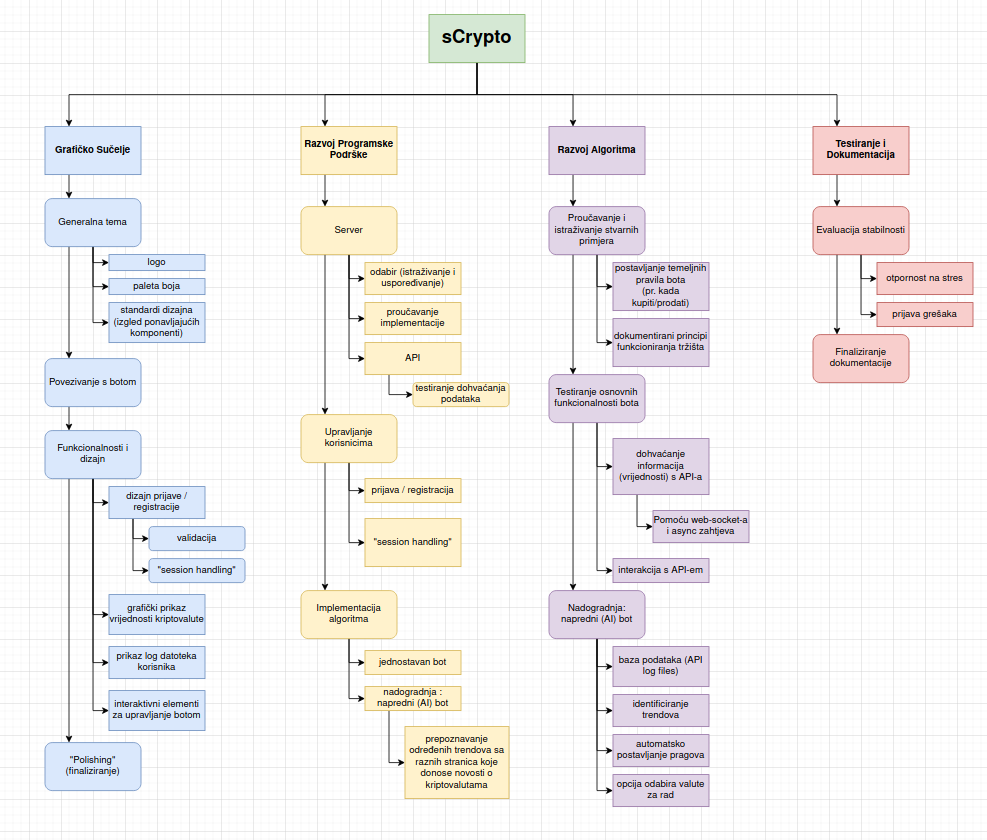
\includegraphics[width=6cm]{wbs}
        \caption{WBS dijagram}
        \label{fig:wbs}
    \end{figure}
\end{frame}

%------------------------------------------------

\begin{frame}{PERT dijagram}
    \begin{itemize}
        \item Određivanje zavisnosti zadataka 
        \item Vrijeme potrebno za izradu
        \item Dozvoljeno kašnjenje zadataka nekritičnog puta
    \end{itemize}
    
\end{frame}

\begin{frame}{PERT dijagram}
    \begin{figure}
        \centering
        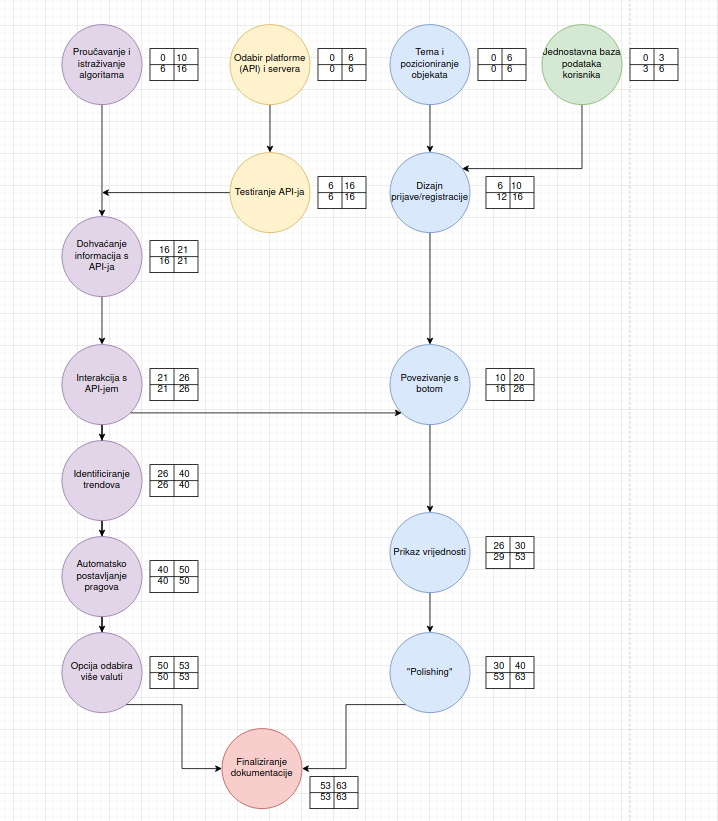
\includegraphics[width=6cm]{pert}
        \caption{Pert diagram}
        \label{fig:pert}
    \end{figure}
\end{frame}

%------------------------------------------------
\section{Platforma i poslužitelj}
%------------------------------------------------

\begin{frame}{Odabir platforme}
    \begin{itemize}
        \item Pronalazak platformi 
        \item Usporedba 
        \item Odabir
    \end{itemize}
\end{frame}

%------------------------------------------------

\begin{frame}{Odabir poslužitelja}
    \begin{itemize}
        \item Pronalazak pogodnih rješenja
        \item Odlučivanje za cloud based poslužitelj
        \item Pronalazak poslužitelja
        \item Usporedba
        \item Odabir
    \end{itemize}
\end{frame}

%------------------------------------------------
\section{Strategija}
%------------------------------------------------

\begin{frame}{Strategija}
    \begin{itemize}
        \item Odabir kriptovalute
        \item Spot vs. leverage trgovanje
        \item Indikatori tehničke analiza
        \item Strategije trgovanja temeljene na indikatorima tehničke analize
        \item Odabir
    \end{itemize}
\end{frame}

%------------------------------------------------
\section{Izrada bota}
%------------------------------------------------

\begin{frame}{Jednostavan bot}
    \begin{itemize}
        \item 2 osnovna stanja - kupi i prodaj
        \item ručni odabir valute
        \item limitirani nalozi
        \end{itemize}
    \end{frame}

%------------------------------------------------

\begin{frame}{Složeni bot}
    \begin{itemize}
        \item AI
        \item provjera stranica s trendovima
        \item naprednije grafičko sučelje
    \end{itemize}
\end{frame}

%------------------------------------------------

\begin{frame}{Poveznica na GitHub repozitorij}
    \begin{itemize}
        \item https://github.com/MSrica/sCrypto\newline
    \end{itemize}
    Članovi: Fran Grenko, Deni Klen, Ani Perušić, Mateo Srića, Karlo Veršić
\end{frame}
%------------------------------------------------

\end{document}